\documentclass[11pt]{article}
\usepackage{graphicx}
\usepackage{caption}
\usepackage{chngcntr}
\usepackage[section]{placeins} % subsections
\usepackage[round, sort, numbers]{natbib}
\usepackage{makecell}
\usepackage{url}
\counterwithin{figure}{section}
\captionsetup[figure]{slc=off}
\usepackage[left=2cm, right=2cm, top=2cm, bottom=2cm]{geometry} % geometry of page
\setcitestyle{square} % square referencing style
\usepackage[fleqn]{amsmath} % for maths
\usepackage{subfig}
\setlength{\parindent}{0pt} % no indents on new paragraphs
\graphicspath{{Code/Analysis/Figures/}}

\begin{document}
\begin{titlepage}
    \begin{center}
        \vspace*{1cm}
        \Huge
        \textbf{Robotics} \\
        \vspace{0.5cm}
        \LARGE
        \vspace{1.5cm}
        \textbf{G. Sheppard, D. Thomas, J. Doering, J. Matthews, C. Li} \\
        \vfill
        \vspace{0.8cm}
        \Large
        University of Birmingham\\
        Physics and Astronomy Department\\
    \end{center}
\end{titlepage}

\tableofcontents

\section{Abstract}
Wow look at \ref{angleplot}. \cite{Bae2006}.

\begin{figure}[!htb]
    \centering
    \captionbox
         {Angleplot.\label{angleplot}}
         {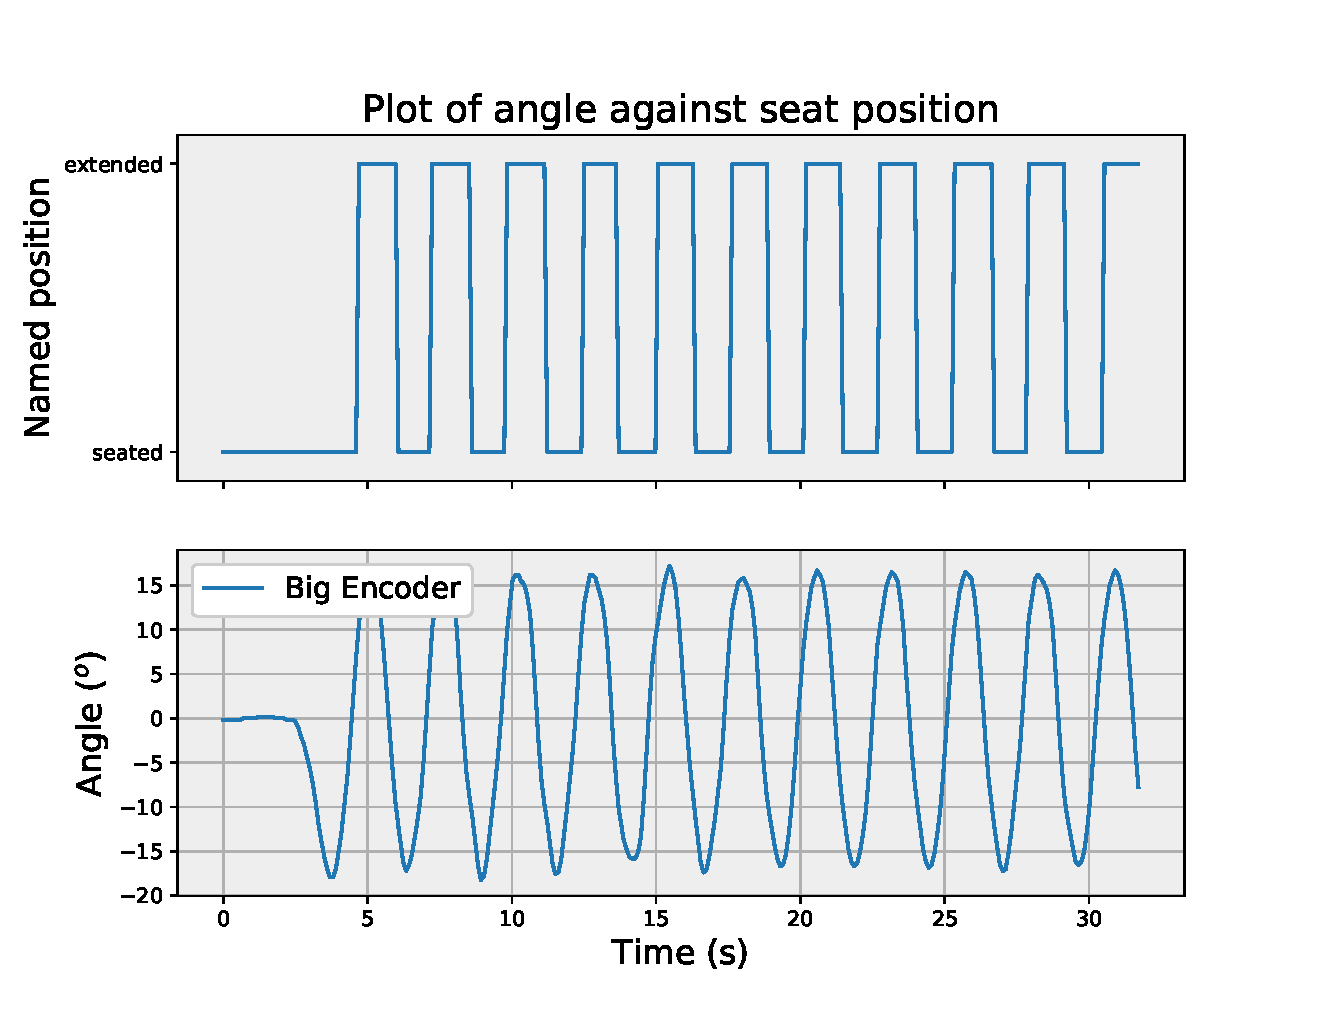
\includegraphics[width=1.0\textwidth]{AnglePlot15-02-201913:29:23}}
\end{figure}

\appendix
\section{Appendix}

\bibliographystyle{ieeetr}
\bibliography{References}
\end{document}